\documentclass{article}
\usepackage{tikz}

\begin{document}
\begin{center}
    
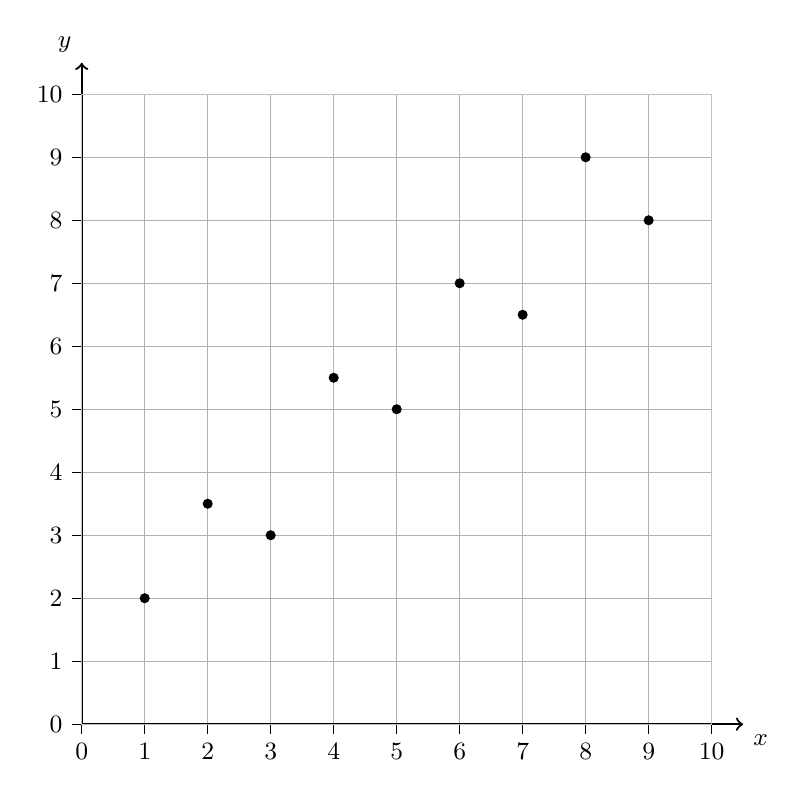
\begin{tikzpicture}[scale=0.8]
  % Styles
  \tikzset{
    pt/.style={fill=black, draw=black, circle, minimum size=4pt, inner sep=0pt},
    axe/.style={->, thick},
  }

  % Grille de fond
  \draw[very thin, color=gray!60, step=1] (0,0) grid (10,10);

  % Axes
  \draw[axe] (0,0) -- (10.5,0) node[below right]{\small $x$};
  \draw[axe] (0,0) -- (0,10.5) node[above left]{\small $y$};

  % Graduations
  \foreach \x in {0,...,10}
    \draw (\x,0) -- (\x,-0.15) node[below] {\small \x};
  \foreach \y in {0,...,10}
    \draw (0,\y) -- (-0.15,\y) node[left] {\small \y};

  % Cadre extérieur
  \draw[gray!50] (0,0) rectangle (10,10);

  % Points
  \foreach \x/\y in {
    1/2,
    2/3.5,
    3/3,
    4/5.5,
    5/5,
    6/7,
    7/6.5,
    8/9,
    9/8
  }{
    \filldraw[pt] (\x,\y) circle (2pt);
  }

\end{tikzpicture}

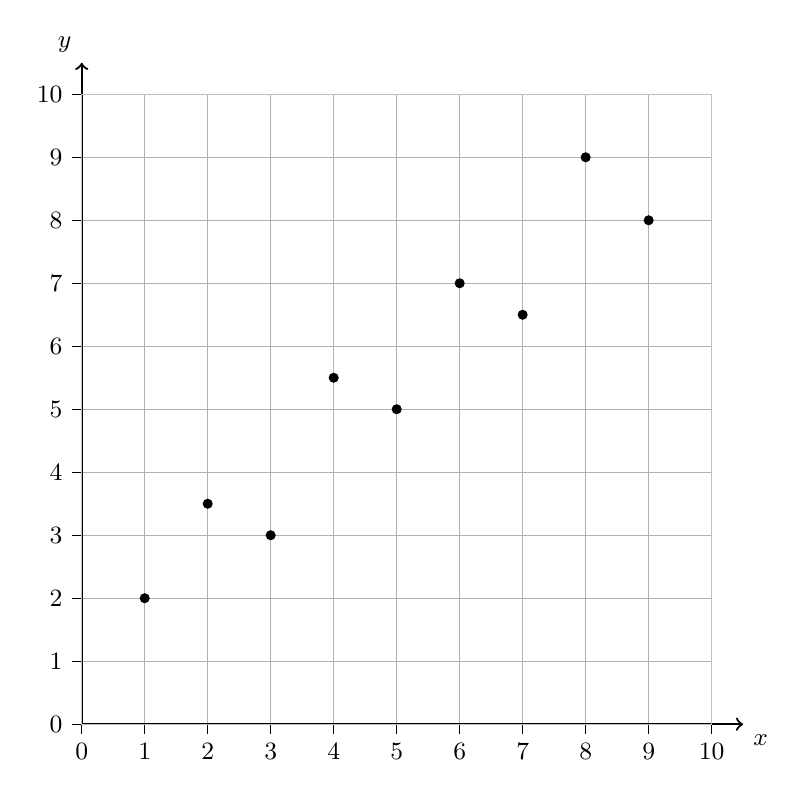
\begin{tikzpicture}[scale=0.8]
  % Styles
  \tikzset{
    pt/.style={fill=black, draw=black, circle, minimum size=4pt, inner sep=0pt},
    axe/.style={->, thick},
  }

  % Grille de fond
  \draw[very thin, color=gray!60, step=1] (0,0) grid (10,10);

  % Axes
  \draw[axe] (0,0) -- (10.5,0) node[below right]{\small $x$};
  \draw[axe] (0,0) -- (0,10.5) node[above left]{\small $y$};

  % Graduations
  \foreach \x in {0,...,10}
    \draw (\x,0) -- (\x,-0.15) node[below] {\small \x};
  \foreach \y in {0,...,10}
    \draw (0,\y) -- (-0.15,\y) node[left] {\small \y};

  % Cadre extérieur
  \draw[gray!50] (0,0) rectangle (10,10);

  % Points
  \foreach \x/\y in {
    1/2,
    2/3.5,
    3/3,
    4/5.5,
    5/5,
    6/7,
    7/6.5,
    8/9,
    9/8
  }{
    \filldraw[pt] (\x,\y) circle (2pt);
  }

\end{tikzpicture}
\end{center}

\end{document}
